\documentclass[11pt]{article}

\usepackage{fullpage}
\usepackage{amsfonts}
\usepackage{graphicx}

\def\eq1{y=\displaystyle{\frac{x}{3x^2+x+1}}}

\def\labelaxes{Remember to include a scale and label your axes}

\begin{document}

\begin{center}
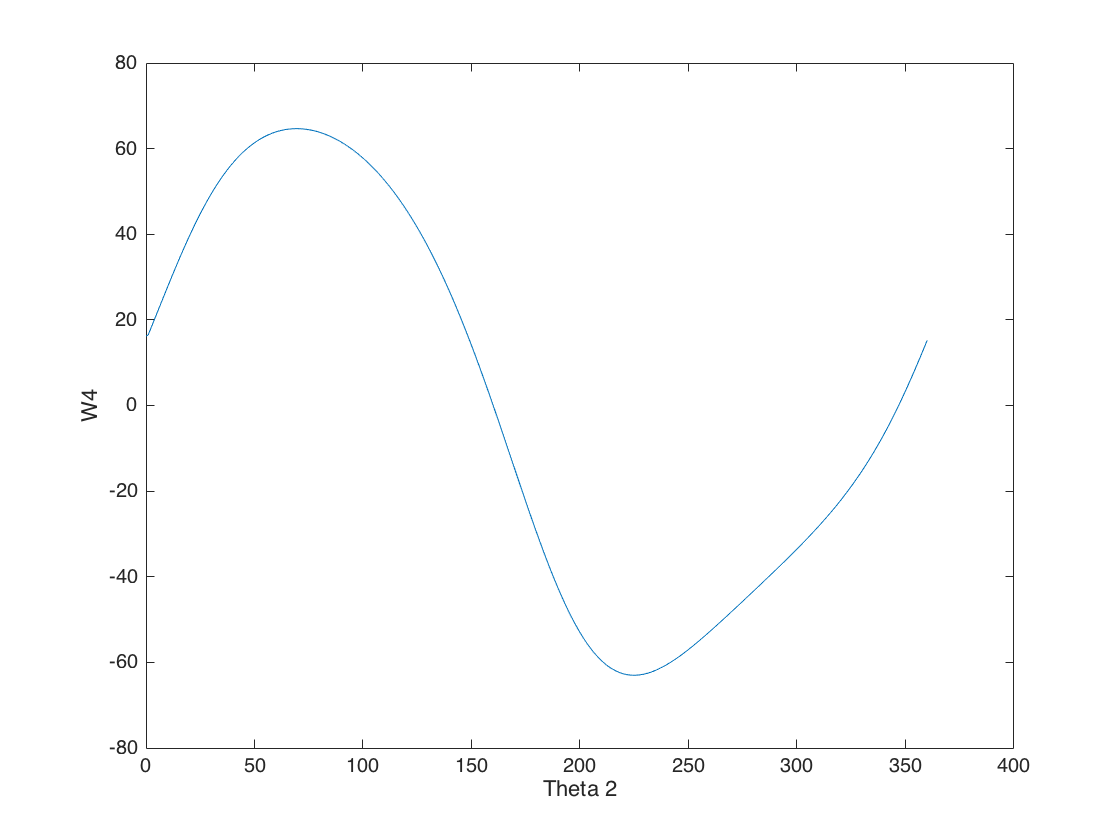
\includegraphics[width=2in]{2vs24.png}
\end{center}


\begin{center}
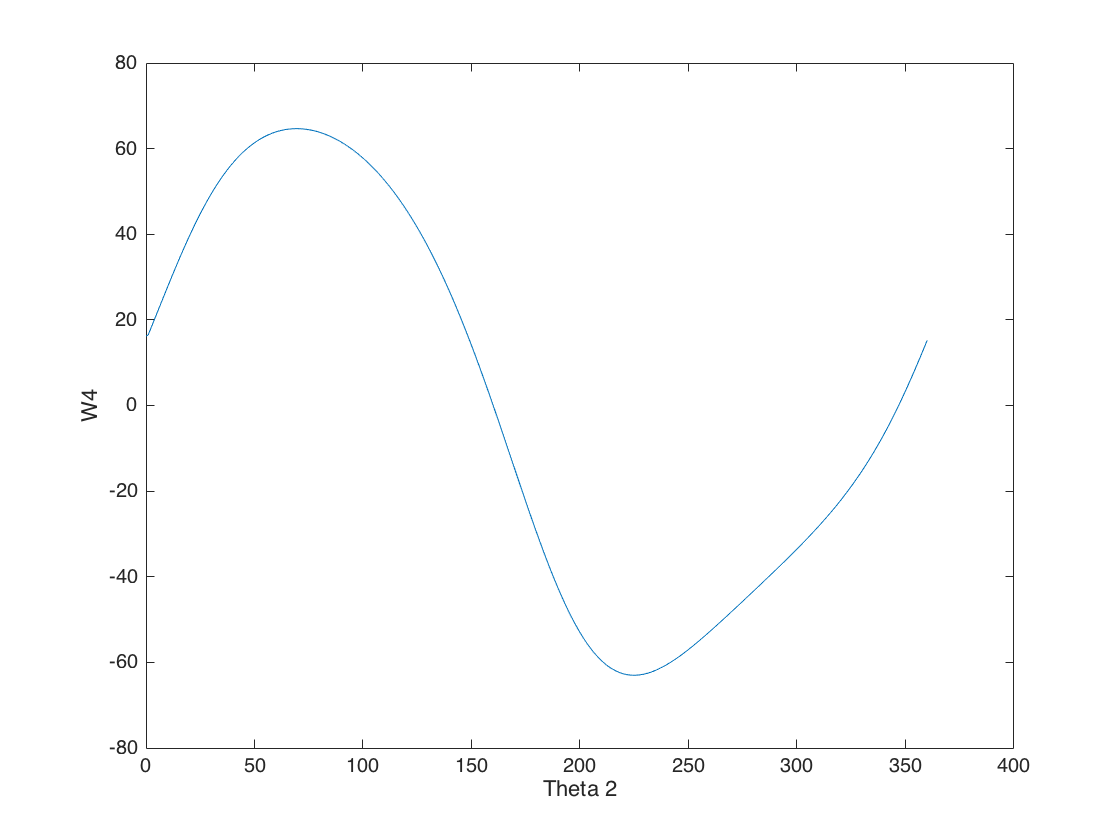
\includegraphics[width=2in,angle=45]{2vs24.png}

Images must be saved as .jpg,.png,.gif or .pdf files.
\end{center}

The set of Natural numbers is denoted by $\mathbb{N}$.

The set of integers is denoted by $\mathbb{Z}$

The set of real numbers is denoted by $\mathbb{R}$

Graph $\eq1$. \labelaxes.

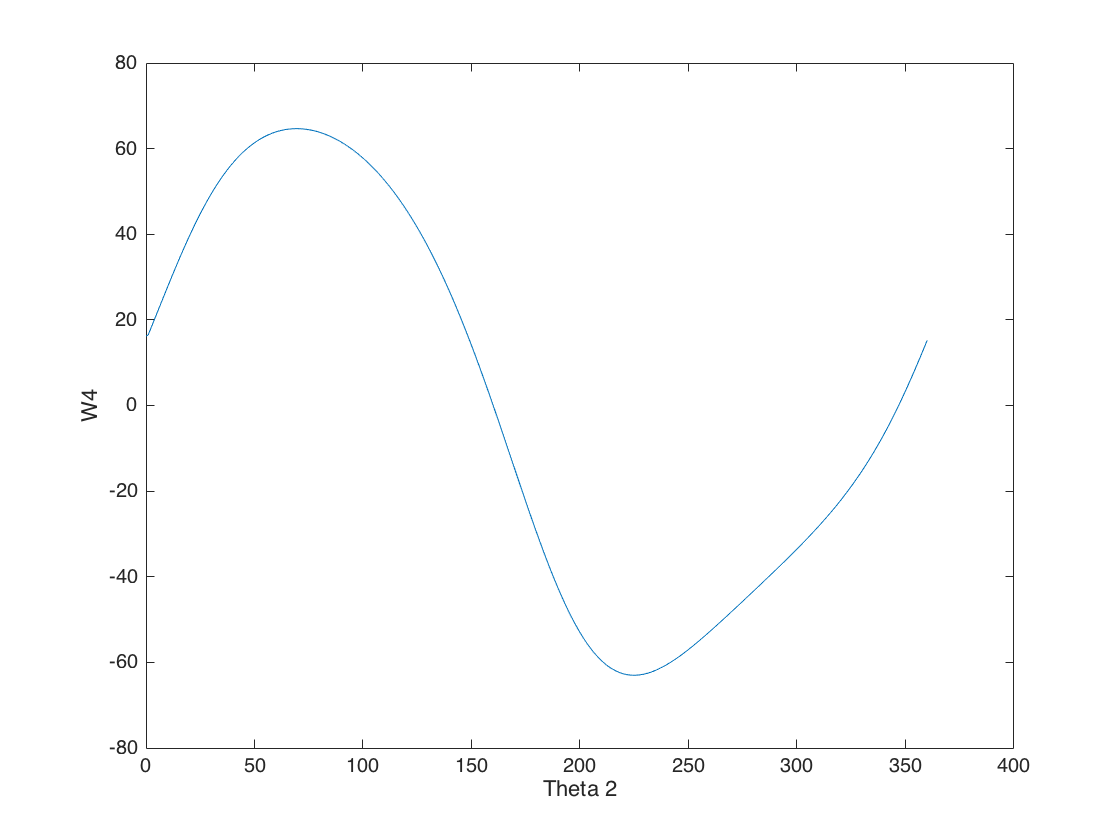
\includegraphics[width=6in]{2vs24.png}

Identify the asymptotes for the graph of $\eq1$.

\end{document}

